%!TEX root = ../../documentation.tex

\section{Requirement conclusion}\label{cha:requirements_conclusion}

The previous sections provide an overview of all requirements for a \ac{MF} application.
This section concludes the overview, by highlighting aspects that stood out.





\subsection{Shell requirements}\label{cha:requirements_conclusion_shellrequirements}

This thesi's root question addresses the shell application, but not all requirements in the previous sections are directly related to the shell.
They are a collection of the expert statements.
Therefore, the following list shows all 19 of 23 requirements which directly affect the shell application.
Generally, all integration requirements, except \textit{\nameref{cha:requirement_detail_integration_crawler}}, affect the shell.

\pagebreak

\begin{itemize}
      \item \textit{\nameref{cha:requirement_detail_integration_loading}}:
            The shell needs to load \acp{MF}, so that they can be integrated

      \item \textit{\nameref{cha:requirement_detail_integration_lifecycle}}:
            If it is required, the shell needs to handle this task

      \item \textit{\nameref{cha:requirement_detail_integration_routing}}:
            The shell is responsible for transitioning between \acp{MF}

      \item \textit{\nameref{cha:requirement_detail_integration_configuration}}:
            The configuration provides the shell the required information, such as where to load a \ac{MF}

      \item \textit{\nameref{cha:requirement_detail_integration_integration}}:
            The shell needs to add a \ac{MF} into the application

      \item \textit{\nameref{cha:requirement_detail_integration_sharedlogic}}:
            The shell can provide common \ac{UI} or logic

      \item \textit{\nameref{cha:requirement_detail_integration_widget}}:
            In case of widgets, the shell might need a pre load feature

      \item \textit{\nameref{cha:requirement_detail_integration_pagelayout}}:
            The shell is responsible to fill the placeholder in this approach

      \item \textit{\nameref{cha:requirement_detail_integration_interoperable}}:
            In order to allow interoperability, there must be an interface for \acp{MF}. The shell uses this interface to work with the \acp{MF}

      \item \textit{\nameref{cha:requirement_detail_integration_abstraction}}:
            This is a specific form of shared logic and therefore the shell is involved

      \item \textit{\nameref{cha:requirement_detail_integration_extensible}}:
            The shell must load the third party extension and integrate them

      \item \hyperref[cha:requirement_detail_performance]{Performance}:
            In this case it is only the feature to provide common dependencies for all \acp{MF} that affects the shell

      \item \textit{\nameref{cha:requirement_detail_state_exchange}}:
            The shell has some responsibility in the approaches, except for the \ac{URL} state exchange approach

      \item \textit{\nameref{cha:requirement_detail_state_intercommunication}}:
            The shell can provide a client communication channel

      \item \textit{\nameref{cha:requirement_detail_state_security}}:
            The authentication process should be handled by the shell

      \item \hyperref[cha:requirement_detail_style]{Consistent style}:
            In case of style isolation, there is an approach that uses a \ac{CSS} namespace per \ac{MF}. The shell needs to handle that

      \item \textit{\nameref{cha:requirement_detail_developer_experience}}:
            Lastly, the common library that the shell could expose
\end{itemize}

The other requirements do not affect the shell for various reasons.
\nameref{cha:requirement_detail_integration_crawler} is a requirement for applications in general and the only restriction it provides is not to use Web Components.
Next is \textit{\nameref{cha:requirement_detail_state_internationalization}}, which is a task for each \ac{MF} and only some form of communication is needed to inform all \acp{MF} about a language change.
Lastly, most of the developer category requirements do not affect the shell, due to the fact, that it is intended for developers.
Autonomy in general affects the shell, but the \textit{\nameref{cha:requirement_detail_developer_autonomy}} requirement focuses on \ac{MF} independence and therefore not on the shell.
The \textit{\nameref{cha:requirement_detail_developer_tools}}, \textit{\nameref{cha:requirement_detail_developer_debugging}} and \textit{\nameref{cha:requirement_detail_developer_testing}} requirements only addresses the development process.
However, \textit{\nameref{cha:requirement_detail_developer_debugging}} proposes a standalone mode for each \ac{MF} which could be realized by a mock shell.
This does not affect the main shell for the application.





\subsection{Shell assessment}\label{cha:requirements_conclusion_shell}

After listing all requirements that are related to the shell, it is also important to point out connections between them.
There are two main connections.
The first is an opposing question in the requirements on whether to focus on a simple or complex shell implementation.
The second is about requirements that are highly likely to require changes in the shell later on.



\paragraph{Simplicity vs. complexity}

The question, whether to focus on simple or complex approaches, was not explicitly mentioned by any experts, but became apparent while uniting the expert opinions for the requirement chapters.
For example, \textciteSteyer{} suggests that the shell should be as slim as possible.
On the other hand, \textcite{Grijzen.2019} proposes to include a templating system that should be handled by the shell.
This is only one example, where experts diverge on the question simplicity vs. complexity.

While the section \ref{cha:requirements_conclusion_shellrequirements} contains all requirements that affect the shell, the Table \ref{tbl:shell_assessment} contains all requirements with their approaches that are connected to the question in no specific order.
The sum of all scores indicates how many approaches are used in favour of complexity rather than simplicity.
So, each requirement has an approach with a score of zero to indicate, that this is the simplest approach for this requirement.
Generally, there are two types of scoring.
The first is, that only one approach within a requirement is possible at the same time.
In this case the approaches are ordered by complexity and scored incrementally.
The second type is that the approaches can coexist and therefore each adds on to the total score of the requirement.
This is indicated by the \enquote{\+1} score.

\begin{table}[h]
      \centering
      \begin{tabular}{|l|l|l|}
            \hline
            \textbf{Requirement} &
            \textbf{Approaches}  &
            \textbf{Score}
            \\ \hline
            \multirow{2}{*}{\nameref{cha:requirement_detail_integration_pagelayout}}
                                 & In use           & 1  \\ \cline{2-3}
                                 & Not in use       & 0  \\ \hline
            \multirow{2}{*}{\nameref{cha:requirement_detail_integration_widget}}
                                 & In use           & 1  \\ \cline{2-3}
                                 & Not in use       & 0  \\ \hline
            \multirow{2}{*}{\nameref{cha:requirement_detail_integration_abstraction}}
                                 & In use           & 1  \\ \cline{2-3}
                                 & Not in use       & 0  \\ \hline
            \multirow{3}{*}{\nameref{cha:requirement_detail_state_exchange}}
                                 & Cache fetch data & 2  \\ \cline{2-3}
                                 & Cache minimal    & 1  \\ \cline{2-3}
                                 & Redux            & 0  \\ \hline
            \multirow{3}{*}{\nameref{cha:requirement_detail_integration_sharedlogic}}
                                 & Business         & +1 \\ \cline{2-3}
                                 & \ac{UI}          & +1 \\ \cline{2-3}
                                 & minimal          & 0  \\ \hline
            \multirow{2}{*}{\nameref{cha:requirement_detail_integration_lifecycle}}
                                 & In use           & 1  \\ \cline{2-3}
                                 & Not in use       & 0  \\ \hline
      \end{tabular}
      \caption{Requirements which affect the shell simplicity vs. complexity including the approach and score}
      \label{tbl:shell_assessment}
\end{table}

This scoring concept only shows the amount of approaches that are used in favour of complexity.
It does not reflect the actual complexity of the shell.
To allow such a comparison, a more sophisticated concept could be to used as a measurement framework, like \textcite{Briand.1996} proposes.



\paragraph{Future change required}

The second aspect that can be outlined is the likelihood of future change in the shell implementation.
The experts have different opinions on whether this should happen or not.
\textciteRehm{} believes that the shell implementation changes over time when new requirements are presented by the developers.
\textciteSteyer{} proposes, that there should even be a separate team for the shell.
On the other hand, \textcite{Laug.2018} advises to implement the shell and then no further changes should occur.
More on these aspects in the \textit{\nameref{cha:requirement_detail_developer_experience}} requirement.

The approaches selected can influence if the shell could need an update later on.
The approaches that are likely to require an update are listed below.
It is important to note, that this also depends on the actual implementation.
Therefore, these are only possible indicators.

\begin{itemize}

      \item \textit{\nameref{cha:requirement_detail_integration_abstraction}}: For example, the browser \ac{API} is updated and therefore the implementation changes. Alternatively, another device is added to the supported platforms, then a new implementation is needed

      \item \textit{\nameref{cha:requirement_detail_state_exchange}}: An example is caching fetched data with the Shell. If the shell caches \ac{API} calls for micro frontends, then changing the \ac{API} could result in a need to update the shell

      \item \textit{\nameref{cha:requirement_detail_integration_sharedlogic}}: For example, a change of shared business logic or a \ac{UI} change.

      \item \textit{\hyperref[cha:requirement_detail_performance]{Performance}}: The depencies change for instance, in case the shell provides shared dependencies for all \acp{MF}.

      \item \textit{\nameref{cha:requirement_detail_developer_experience}}: A new feature is needed for example while the shell provides a library with common functions.

\end{itemize}





\subsection{Requirement overlapping approaches}

Two approaches stood out compared to other approaches, because they can be used to fulfill or support multiple requirements.
The first one is a common feature library and the second is using the browser feature Web Components.



\paragraph{Common feature library}\label{cha:requirements_conclusion_commonlibrary}

A common feature library contains commonly needed functionalities, such as navigating to another \ac{URL}, emitting an event or abstracting a browser feature.
The abstraction is used to allow reusing \acp{MF} for multiple browsers, where the \ac{API} varies.
Also, the complexity of these functions vary.
A simple functionality for instance is emitting an event, where a simple function uses the browser \ac{API} to send a custom event.
On the other hand, providing an abstraction layer for the browser \ac{API} includes browser specific loading of function implementations.
The common feature library could either be shared by the shell via a global variable or a library which needs to be included in each \ac{MF}.
Which approach is used, depends on the functionalities in the common library.

The requirements \textit{\nameref{cha:requirement_detail_integration_routing}}, \textit{\nameref{cha:requirement_detail_integration_sharedlogic}}, \textit{\nameref{cha:requirement_detail_state_exchange}}, \textit{\nameref{cha:requirement_detail_integration_abstraction}}, \textit{\nameref{cha:requirement_detail_state_intercommunication}}, \textit{\nameref{cha:requirement_detail_state_security}} and \hyperref[cha:requirement_detail_style]{Consistent style} could contribute functionalities to the common library.
This library would also be beneficial to the \textit{\nameref{cha:requirement_detail_integration_extensible}} and \textit{\nameref{cha:requirement_detail_developer_experience}} requirements.



\paragraph{Web Components}\label{cha:requirements_conclusion_webcomponents}

Another reoccurring approach is the browser feature Web Components.
Using this approach has mainly two downsides.
First, it is not fully supported by all browsers.
In this case polyfills can help, but there are also browsers where it does not work with polyfills.
For example, in console or smart TV browsers.
More on that in the \textit{\nameref{cha:requirement_detail_integration_integration}} requirement.
The second downside is, that if Web Components are used in combination with their shadow \ac{DOM} feature, it is not indexable by current search engine browsers.
More on that in the \textit{\nameref{cha:requirement_detail_integration_crawler}} requirement.

If these downsides do not matter for the project, Web Components offer following advantages:
The feature shadow \ac{DOM} allows to fully isolate styles, see \textit{\hyperref[cha:requirement_detail_style]{Consistent style}}.
A Web Component is also able to encapsulate frameworks within them, therefore allowing technology agnostic \acp{MF}, see also \textit{\nameref{cha:requirement_detail_developer_autonomy}}.
Besides the isolation capabilities, it also provides an interface to pass information into the Web Component using \ac{HTML} attributes or \ac{JS} properties.
This is a browser native solution to handle state, see \textit{\nameref{cha:requirement_detail_state_exchange}}.
The final advantage is that it is a simple implementation for the \textit{\nameref{cha:requirement_detail_integration_widget}} requirement.





\subsection{Application assessment}\label{cha:requirements_conclusion_application}

The requirements also contain a more general opposing question on whether to focus on autonomy or performance in a \ac{MF} application.
This question was also mentioned by \textciteSteyer{}.
In general, the more autonomy approaches are used the bigger the application will be.
The impact of the application size is outlined in the \textit{\hyperref[cha:requirement_detail_performance]{Performance}} requirement.
It is important to point out, that only because the used approaches favour autonomy, this does not imply a bad performance.
Instead, it provides extra stress on the end user's devices, mainly because of larger \ac{JS} sizes and amount of frameworks used in the application.

The Table \ref{tbl:application_assessment} contains all requirements that are connected to the question.
The Table structure is the same as in \textit{\ref{cha:requirements_conclusion_shell}}.
As in the other section, the score is added to make \ac{MF} applications comparable.
A score of zero here indicates autonomy and the higher the score, the higher the focus on performance.
Therefore, a low score indicates, that the application uses a more autonomy focused implementation then performance and vice versa.

The score of some approaches need an explanation.
For example, the \textit{\nameref{cha:requirement_detail_integration_abstraction}} requirement can either be used or not.
If it is used, then there is a central point to handle abstraction, therefore reducing the amount of code.
On the other hand, it creates coupling between the \ac{MF} and shell, while reducing coupling between the \ac{MF} and browser \ac{API}.
Consequently, score 0 indicates more of a neutral approach whereas 1 slightly leans towards performance.
Another example is the \textit{\nameref{cha:requirement_detail_integration_pagelayout}} requirement.
Its score is inverted compared to other requirements.
The reason being, that if multiple micro frontends are allowed in the same page, then this could result in a performance problem.
On the other hand, autonomy is fully supported, because the developers are free in designing pages as they need it.
Therefore, it is a performance gain not to use the \textit{\nameref{cha:requirement_detail_integration_pagelayout}} approach as it reduces the developers freedom.


\begin{table}[h]
      \centering
      \begin{tabular}{|l|l|l|}
            \hline
            \textbf{Requirement} &
            \textbf{Approach}    &
            \textbf{Score}
            \\ \hline
            \multirow{2}{*}{\nameref{cha:requirement_detail_integration_pagelayout}}
                                 & In use                                    & 0                             \\ \cline{2-3}
                                 & Not in use                                & 1                             \\ \hline
            \multirow{2}{*}{\nameref{cha:requirement_detail_integration_widget}}
                                 & In use                                    & 1                             \\ \cline{2-3}
                                 & Not in use                                & 0                             \\ \hline
            \multirow{2}{*}{\nameref{cha:requirement_detail_integration_abstraction}}
                                 & In use                                    & 1                             \\ \cline{2-3}
                                 & Not in use                                & 0                             \\ \hline
            \multirow{3}{*}{\nameref{cha:requirement_detail_state_exchange}}
                                 & Redux                                     & 2                             \\ \cline{2-3}
                                 & Cache fetch data                          & 1                             \\ \cline{2-3}
                                 & Cache minimal                             & 0                             \\ \hline
            \multirow{3}{*}{\nameref{cha:requirement_detail_integration_sharedlogic}}
                                 & Business                                  & +1                            \\ \cline{2-3}
                                 & \ac{UI}                                   & +1                            \\ \cline{2-3}
                                 & Minimal                                   & 0                             \\ \hline
            \multirow{3}{*}{\makecell[l]{\textit{\hyperref[cha:requirement_detail_performance]{Performance}} \\ (shared dependencies)}}
                                 & Many                                      & 2                             \\ \cline{2-3}
                                 & Few                                       & 1                             \\ \cline{2-3}
                                 & Non                                       & 0                             \\ \hline
            \multirow{3}{*}{\makecell[l]{\textit{\hyperref[cha:requirement_detail_performance]{Performance}} \\ (shared core)}}
                                 & One framework                             & 2                             \\ \cline{2-3}
                                 & Multiple frameworks or framework versions & 1                             \\ \cline{2-3}
                                 & No core sharing                           & 0                             \\ \hline
      \end{tabular}
      \caption{Requirements which affect the application autonomy or performance including the approach and score}
      \label{tbl:application_assessment}
\end{table}




\subsection{Assessment overview}\label{cha:requirements_conclusion_assessment}

Two similar methods to measure the affiliation of the shell and the \ac{MF} application itself to attitudes are proposed in \ref{cha:requirements_conclusion_shell} and \ref{cha:requirements_conclusion_application}.
They can be combined into one chart, shown in Figure \ref{img:quadrant_chart}.
The shell's opposing question covers a range from 0 (simple) to 8 (complex)on the vertical axis of the graph.
The horizontal axis is the application's opposing question, that covers a range from 0 (autonomy) to 11 (performance).

\begin{figure}[h]
      \centering
      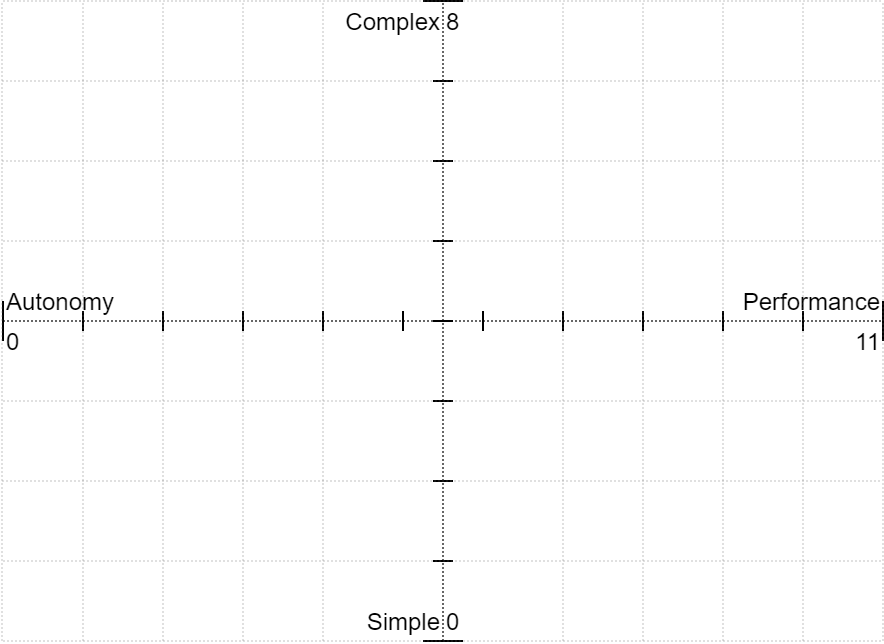
\includegraphics[scale=0.5]{quadrant_chart.png}
      \caption{Quadrant chart of the opposing questions, simplicity vs. complexity, and autonomy vs. performance}
      \label{img:quadrant_chart}
\end{figure}

The graph can be used to compare applications in one image.
It provides an overview of the driving affiliations for an application.
Both assessment Tables \ref{tbl:application_assessment} and \ref{tbl:shell_assessment} only reflect the amount of approaches taken into a certain direction, rather than actually outlining how strong an application invests into any of the directions.
Therefore, it is hard to determine the significance of this chart, but it is a first approach on providing an overview.





\subsection{Analysis conclusion}

The requirement analysis resulted in 23 requirements and many approaches.
To better outline which of the requirements are actually important, they are firstly grouped into categories.
These categories were then ordered by importance, see \ref{cha:requirement_categories}.
After that, the requirements within each categories were ordered by importance, see \ref{cha:requirements_overview}.
Finally, each requirement with their approaches are explained, which resulted in many cross-references and partially overlapping information.
Therefore, the section \ref{cha:requirements_conclusion} outlines important facts that became apparent while working on the requirement analysis.
The section \ref{cha:requirements_conclusion_assessment} is used in the next chapter to compare different applications against each other.
